\subsection{Problem 3.2. More Transportation Schedules}

\begin{figure}[H]
	\centering
	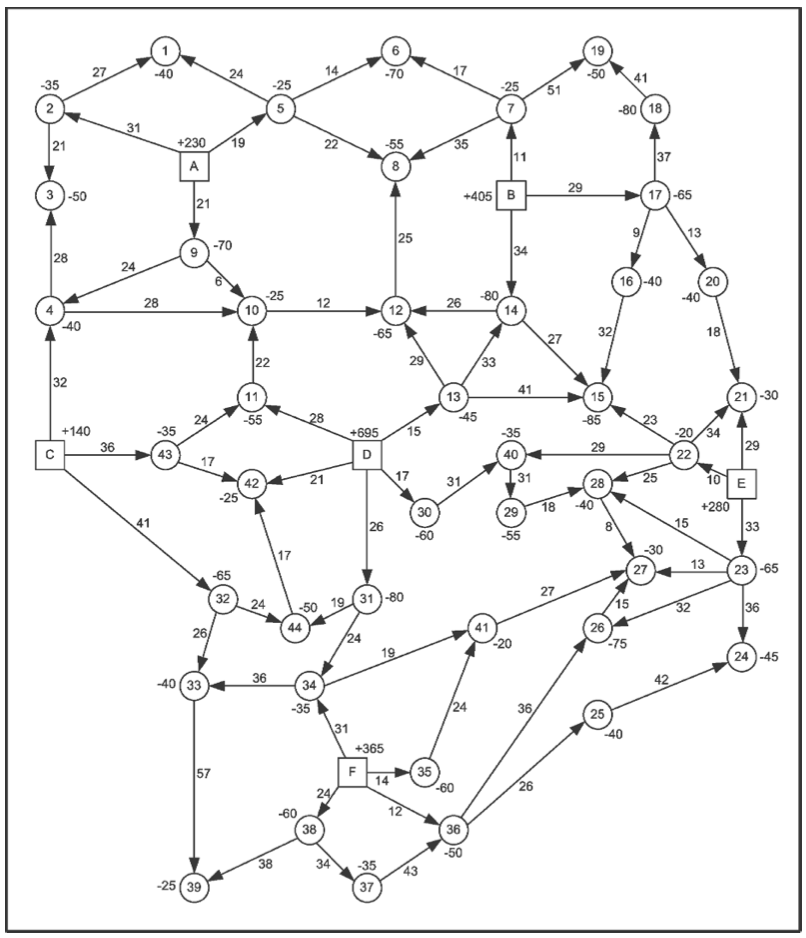
\includegraphics[scale=1]{./img/figure3-14.png}
	\caption{Supplies and demands (in units of 10 spools), and truck costs (in units of e10) on a road map with 50 locations}
	\label{network3-2}
\end{figure}

\paragraph{}
\begin{quote}
In another country GTC has to deal with similar questions as in Problem 3.1. In Figure \ref{network3-2} the road map for this country is depicted with 50 locations. There are six cable depots, labeled A, B, C, D, E, and F. All numbers in this figure are given in units of ten spools. The inventories at the various depots are the positive numbers next to the depot labels. For instance, in depot C there are 1,400 cable spools in stock. The locations with labels 1,~\dots,~44 are points where cable is needed, so called demand locations. The numbers next to these labels (with a negative sign) refer to the number of spools demanded at these points. For instance, 650 spools needed at location 17. The numbers attached to the road segments are the transportation costs (in \texteuro 10 units). For instance, the cost of transporting ten spools with one truck is \texteuro 290 on the road segment 22 $\rightarrow$ 40.
\end{quote}

\paragraph{(a)}
\begin{quote}
Determine a transportation plan such that all demands are satisfied at minimum truck costs.
\end{quote}

\paragraph{}
\paragraph{}
We find the minimum cost maximum flow in a network obtained from figure \ref{network3-2}. The capacities of arcs are infinite, the costs are taken from figure \ref{network3-2}. To 50 existing vertices we added a source and a sink. We added arcs from source to the 6 depots with zero costs and capacities equal to the number of spools in depots. We added arcs from all demand locations to sink with zero costs and capacities equal to the number of demanded spools. We found minimum cost maximum flow and checked that it has saturated all arcs to the sink (i.e. all demand is satisfied).

\paragraph{}
Each arc (except the arcs incident to sink or source) in our graph corresponds to a road. The flow through an arc in our graph corresponds to the number of spools transported through it. The arcs from source spread incoming flow among depots and limit the flow from each depot. The arcs to sink aggregate the flow from demand locations and limit the demand of each location. The flow through edges can be used as a transportation plan right away. It can be more convenient to have a transportation plan as a list of routes from source depots to demand locations, so that a truck can be assigned to each route. We found both representations. We obtained the second representation from the first one using greedy algorithm.

\paragraph{}
The flow as a list of flows through edges is shown in figure \ref{flow3-2a}. The transportation plan as a list of routes is shown in table \ref{flow3-2a-paths}. The minimum total cost is \texteuro 831,800.

\begin{figure}[H]
\centering
\begin{multicols}{5}
$ 2 \rightarrow 3 $ : 50

$ 5 \rightarrow 1 $ : 40

$ 5 \rightarrow 8 $ : 10

$ 7 \rightarrow 6 $ : 70

$ 7 \rightarrow 8 $ : 35

$ 7 \rightarrow 19 $ : 50
$ 11 \rightarrow 10 $ : 25
$ 12 \rightarrow 8 $ : 10
$ 13 \rightarrow 12 $ : 75
$ 13 \rightarrow 14 $ : 80
$ 13 \rightarrow 15 $ : 35
$ 17 \rightarrow 16 $ : 40
$ 17 \rightarrow 18 $ : 80
$ 17 \rightarrow 20 $ : 40
$ 22 \rightarrow 15 $ : 50
$ 22 \rightarrow 28 $ : 70
$ 23 \rightarrow 24 $ : 45
$ 28 \rightarrow 27 $ : 30
$ 30 \rightarrow 40 $ : 90
$ 31 \rightarrow 34 $ : 75
$ 31 \rightarrow 44 $ : 50
$ 34 \rightarrow 33 $ : 40
$ 35 \rightarrow 41 $ : 20
$ 36 \rightarrow 25 $ : 40
$ 36 \rightarrow 26 $ : 75
$ 38 \rightarrow 37 $ : 35
$ 38 \rightarrow 39 $ : 25
$ 40 \rightarrow 29 $ : 55
$ 45 \rightarrow 2 $ : 85
$ 45 \rightarrow 5 $ : 75
$ 45 \rightarrow 9 $ : 70
$ 46 \rightarrow 7 $ : 180
$ 46 \rightarrow 17 $ : 225
$ 47 \rightarrow 4 $ : 40
$ 47 \rightarrow 32 $ : 65
$ 47 \rightarrow 43 $ : 35
$ 48 \rightarrow 11 $ : 80
$ 48 \rightarrow 13 $ : 235
$ 48 \rightarrow 30 $ : 150
$ 48 \rightarrow 31 $ : 205
$ 48 \rightarrow 42 $ : 25
$ 49 \rightarrow 21 $ : 30
$ 49 \rightarrow 22 $ : 140
$ 49 \rightarrow 23 $ : 110
$ 50 \rightarrow 35 $ : 80
$ 50 \rightarrow 36 $ : 165
$ 50 \rightarrow 38 $ : 120
\end{multicols}
\caption{Optimal transportation plan: the flow through each arc in tens of spools}
\label{flow3-2a}
\end{figure}

\begin{table}[H]
\centering
\begin{tabular}{|r|l|l|}
\hline
Path & Tens of spools & Cost \\ \hline
$ A \rightarrow 2 $ & 35 & \texteuro 1085\\ \hline
$ A \rightarrow 2 \rightarrow 3 $ & 50 & \texteuro 2600\\ \hline
$ A \rightarrow 5 $ & 25 & \texteuro 475\\ \hline
$ A \rightarrow 5 \rightarrow 1 $ & 40 & \texteuro 1720\\ \hline
$ A \rightarrow 5 \rightarrow 8 $ & 10 & \texteuro 410\\ \hline
$ A \rightarrow 9 $ & 70 & \texteuro 1470\\ \hline
$ B \rightarrow 7 $ & 25 & \texteuro 275\\ \hline
$ B \rightarrow 7 \rightarrow 6 $ & 70 & \texteuro 1960\\ \hline
$ B \rightarrow 7 \rightarrow 8 $ & 35 & \texteuro 1610\\ \hline
$ B \rightarrow 7 \rightarrow 19 $ & 50 & \texteuro 3100\\ \hline
$ B \rightarrow 17 $ & 65 & \texteuro 1885\\ \hline
$ B \rightarrow 17 \rightarrow 16 $ & 40 & \texteuro 1520\\ \hline
$ B \rightarrow 17 \rightarrow 18 $ & 80 & \texteuro 5280\\ \hline
$ B \rightarrow 17 \rightarrow 20 $ & 40 & \texteuro 1680\\ \hline
$ C \rightarrow 4 $ & 40 & \texteuro 1280\\ \hline
$ C \rightarrow 32 $ & 65 & \texteuro 2665\\ \hline
$ C \rightarrow 43 $ & 35 & \texteuro 1260\\ \hline
$ D \rightarrow 11 $ & 55 & \texteuro 1540\\ \hline
$ D \rightarrow 11 \rightarrow 10 $ & 25 & \texteuro 1250\\ \hline
$ D \rightarrow 13 $ & 45 & \texteuro 675\\ \hline
$ D \rightarrow 13 \rightarrow 12 $ & 65 & \texteuro 2860\\ \hline
$ D \rightarrow 13 \rightarrow 12 \rightarrow 8 $ & 10 & \texteuro 690\\ \hline
$ D \rightarrow 13 \rightarrow 14 $ & 80 & \texteuro 3840\\ \hline
$ D \rightarrow 13 \rightarrow 15 $ & 35 & \texteuro 1960\\ \hline
$ D \rightarrow 30 $ & 60 & \texteuro 1020\\ \hline
$ D \rightarrow 30 \rightarrow 40 $ & 35 & \texteuro 1680\\ \hline
$ D \rightarrow 30 \rightarrow 40 \rightarrow 29 $ & 55 & \texteuro 4345\\ \hline
$ D \rightarrow 31 $ & 80 & \texteuro 2080\\ \hline
$ D \rightarrow 31 \rightarrow 34 $ & 35 & \texteuro 1750\\ \hline
$ D \rightarrow 31 \rightarrow 34 \rightarrow 33 $ & 40 & \texteuro 3440\\ \hline
$ D \rightarrow 31 \rightarrow 44 $ & 50 & \texteuro 2250\\ \hline
$ D \rightarrow 42 $ & 25 & \texteuro 525\\ \hline
$ E \rightarrow 21 $ & 30 & \texteuro 870\\ \hline
$ E \rightarrow 22 $ & 20 & \texteuro 200\\ \hline
$ E \rightarrow 22 \rightarrow 15 $ & 50 & \texteuro 1650\\ \hline
$ E \rightarrow 22 \rightarrow 28 $ & 40 & \texteuro 1400\\ \hline
$ E \rightarrow 22 \rightarrow 28 \rightarrow 27 $ & 30 & \texteuro 1290\\ \hline
$ E \rightarrow 23 $ & 65 & \texteuro 2145\\ \hline
$ E \rightarrow 23 \rightarrow 24 $ & 45 & \texteuro 3105\\ \hline
$ F \rightarrow 35 $ & 60 & \texteuro 840\\ \hline
$ F \rightarrow 35 \rightarrow 41 $ & 20 & \texteuro 760\\ \hline
$ F \rightarrow 36 $ & 50 & \texteuro 600\\ \hline
$ F \rightarrow 36 \rightarrow 25 $ & 40 & \texteuro 1520\\ \hline
$ F \rightarrow 36 \rightarrow 26 $ & 75 & \texteuro 3600\\ \hline
$ F \rightarrow 38 $ & 60 & \texteuro 1440\\ \hline
$ F \rightarrow 38 \rightarrow 37 $ & 35 & \texteuro 2030\\ \hline
$ F \rightarrow 38 \rightarrow 39 $ & 25 & \texteuro 1550\\ \hline
\end{tabular}
\caption{Optimal transportation plan decomposed into paths}
\label{flow3-2a-paths}
\end{table}

\paragraph{(b)}
\begin{quote}
It is observed that unacceptable situations occur when trucks arrive from different directions at demand locations. Is it possible to make a feasible transportation plan such that all demands are satisfied and the unacceptable situations are avoided? Explain your answer.
\end{quote}

\paragraph{}
The total number of spools in stock is equal to the total demand. So each depot has to get rid of all spools. To avoid the unacceptable, each demand location must have exactly one ingoing edge with positive flow. This means that the subgraph of edges with non-zero flow must consist of six disjoint trees rooted at the depots. All arcs of the trees must be oriented away from root. The sum of demands in a tree must be equal to the number of spools in stock of its depot.

\paragraph{}
Let's show it's impossible for the given network. Consider the depot B. It has capacity 405. Vertices 7, 16,17,18,19,20 are only reachable from B, so they have to belong to B's tree. This leaves $405-25-40-65-80-50-40=105$ units of capacity in B. It can be seen that it's impossible to add some vertices with total demand $105$ to the tree (there are so few combinations they can be checked manually).

\paragraph{(c)}
\begin{quote}
If the answer to the previous question is ``no'', how will you change the inventories (supplies) in the various depots so that such a plan can be constructed.
\end{quote}

\paragraph{}
Let's find the minimum possible total cost that can be obtained in this network by adding spools to depots. To do this we increase source capacities to infinity and find the minimum cost maximum flow. Then we can find the required number of spools in each depot as the flow through the edge from source to this depot. Such flow will always consist of disjoint trees (if we omit the source) because it essentially becomes the tree of shortest paths from source to all other vertices.

\paragraph{}
The resulting increased supplies are shown in table \ref{increased-supplies}. The flow as a list of flows through edges is shown in figure \ref{flow3-2c}. The transportation plan as a list of routes is shown in table \ref{flow3-2c-paths}. The resulting total cost is \texteuro 776,650.

\begin{table}[H]
\centering
\begin{tabular}{|c|c|c|c|c|c|}
\hline
A & B & C & D & E & F \\ \hline
365 & 450 & 180 & 695 & 405 & 400  \\ \hline
\end{tabular}
\caption{Increased supplies in each depot in tens of spools}
\label{increased-supplies}
\end{table}

\begin{figure}[H]
\centering
\begin{multicols}{5}
$ 2 \rightarrow 3 $ : 50

$ 5 \rightarrow 1 $ : 40

$ 5 \rightarrow 8 $ : 55

$ 7 \rightarrow 6 $ : 70

$ 7 \rightarrow 19 $ : 50
$ 9 \rightarrow 10 $ : 90
$ 10 \rightarrow 12 $ : 65
$ 17 \rightarrow 16 $ : 40
$ 17 \rightarrow 18 $ : 80
$ 17 \rightarrow 20 $ : 40
$ 22 \rightarrow 15 $ : 85
$ 22 \rightarrow 28 $ : 70
$ 22 \rightarrow 40 $ : 90
$ 23 \rightarrow 24 $ : 45
$ 28 \rightarrow 27 $ : 30
$ 31 \rightarrow 44 $ : 50
$ 32 \rightarrow 33 $ : 40
$ 35 \rightarrow 41 $ : 20
$ 36 \rightarrow 25 $ : 40
$ 36 \rightarrow 26 $ : 75
$ 38 \rightarrow 37 $ : 35
$ 38 \rightarrow 39 $ : 25
$ 40 \rightarrow 29 $ : 55
$ 45 \rightarrow 2 $ : 85
$ 45 \rightarrow 5 $ : 120
$ 45 \rightarrow 9 $ : 160
$ 46 \rightarrow 7 $ : 145
$ 46 \rightarrow 14 $ : 80
$ 46 \rightarrow 17 $ : 225
$ 47 \rightarrow 4 $ : 40
$ 47 \rightarrow 32 $ : 105
$ 47 \rightarrow 43 $ : 35
$ 48 \rightarrow 11 $ : 55
$ 48 \rightarrow 13 $ : 45
$ 48 \rightarrow 30 $ : 60
$ 48 \rightarrow 31 $ : 130
$ 48 \rightarrow 42 $ : 25
$ 49 \rightarrow 21 $ : 30
$ 49 \rightarrow 22 $ : 265
$ 49 \rightarrow 23 $ : 110
$ 50 \rightarrow 34 $ : 35
$ 50 \rightarrow 35 $ : 80
$ 50 \rightarrow 36 $ : 165
$ 50 \rightarrow 38 $ : 120
\end{multicols}
\caption{Optimal transportation plan: the flow through each arc in tens of spools}
\label{flow3-2c}
\end{figure}

\begin{table}[H]
\centering
\begin{tabular}{|r|l|l|}
\hline
Path & Tens of spools & Cost \\ \hline
$ A \rightarrow 2 $ & 35 & \texteuro 1085\\ \hline
$ A \rightarrow 2 \rightarrow 3 $ & 50 & \texteuro 2600\\ \hline
$ A \rightarrow 5 $ & 25 & \texteuro 475\\ \hline
$ A \rightarrow 5 \rightarrow 1 $ & 40 & \texteuro 1720\\ \hline
$ A \rightarrow 5 \rightarrow 8 $ & 55 & \texteuro 2255\\ \hline
$ A \rightarrow 9 $ & 70 & \texteuro 1470\\ \hline
$ A \rightarrow 9 \rightarrow 10 $ & 25 & \texteuro 675\\ \hline
$ A \rightarrow 9 \rightarrow 10 \rightarrow 12 $ & 65 & \texteuro 2535\\ \hline
$ B \rightarrow 7 $ & 25 & \texteuro 275\\ \hline
$ B \rightarrow 7 \rightarrow 6 $ & 70 & \texteuro 1960\\ \hline
$ B \rightarrow 7 \rightarrow 19 $ & 50 & \texteuro 3100\\ \hline
$ B \rightarrow 14 $ & 80 & \texteuro 2720\\ \hline
$ B \rightarrow 17 $ & 65 & \texteuro 1885\\ \hline
$ B \rightarrow 17 \rightarrow 16 $ & 40 & \texteuro 1520\\ \hline
$ B \rightarrow 17 \rightarrow 18 $ & 80 & \texteuro 5280\\ \hline
$ B \rightarrow 17 \rightarrow 20 $ & 40 & \texteuro 1680\\ \hline
$ C \rightarrow 4 $ & 40 & \texteuro 1280\\ \hline
$ C \rightarrow 32 $ & 65 & \texteuro 2665\\ \hline
$ C \rightarrow 32 \rightarrow 33 $ & 40 & \texteuro 2680\\ \hline
$ C \rightarrow 43 $ & 35 & \texteuro 1260\\ \hline
$ D \rightarrow 11 $ & 55 & \texteuro 1540\\ \hline
$ D \rightarrow 13 $ & 45 & \texteuro 675\\ \hline
$ D \rightarrow 30 $ & 60 & \texteuro 1020\\ \hline
$ D \rightarrow 31 $ & 80 & \texteuro 2080\\ \hline
$ D \rightarrow 31 \rightarrow 44 $ & 50 & \texteuro 2250\\ \hline
$ D \rightarrow 42 $ & 25 & \texteuro 525\\ \hline
$ E \rightarrow 21 $ & 30 & \texteuro 870\\ \hline
$ E \rightarrow 22 $ & 20 & \texteuro 200\\ \hline
$ E \rightarrow 22 \rightarrow 15 $ & 85 & \texteuro 2805\\ \hline
$ E \rightarrow 22 \rightarrow 28 $ & 40 & \texteuro 1400\\ \hline
$ E \rightarrow 22 \rightarrow 28 \rightarrow 27 $ & 30 & \texteuro 1290\\ \hline
$ E \rightarrow 22 \rightarrow 40 $ & 35 & \texteuro 1365\\ \hline
$ E \rightarrow 22 \rightarrow 40 \rightarrow 29 $ & 55 & \texteuro 3850\\ \hline
$ E \rightarrow 23 $ & 65 & \texteuro 2145\\ \hline
$ E \rightarrow 23 \rightarrow 24 $ & 45 & \texteuro 3105\\ \hline
$ F \rightarrow 34 $ & 35 & \texteuro 1085\\ \hline
$ F \rightarrow 35 $ & 60 & \texteuro 840\\ \hline
$ F \rightarrow 35 \rightarrow 41 $ & 20 & \texteuro 760\\ \hline
$ F \rightarrow 36 $ & 50 & \texteuro 600\\ \hline
$ F \rightarrow 36 \rightarrow 25 $ & 40 & \texteuro 1520\\ \hline
$ F \rightarrow 36 \rightarrow 26 $ & 75 & \texteuro 3600\\ \hline
$ F \rightarrow 38 $ & 60 & \texteuro 1440\\ \hline
$ F \rightarrow 38 \rightarrow 37 $ & 35 & \texteuro 2030\\ \hline
$ F \rightarrow 38 \rightarrow 39 $ & 25 & \texteuro 1550\\ \hline
\end{tabular}
\caption{Optimal transportation plan decomposed into paths}
\label{flow3-2c-paths}
\end{table}

\paragraph{(d)}
\begin{quote}
Also try to construct a transportation plan without the unacceptable situations, by changing the traffic direction on certain road segments.
\end{quote}

\paragraph{}
Consider the following problem. We have a network, where some vertices are sources and all the other vertices are sinks. The sources and sinks have capacities, and the total capacity of sources is equal to the total capacity of sinks. The edges have no orientation and cost and have infinite capacity. We need to find a flow saturating all sources and sinks such that no sink has more than one ingoing edge with positive flow. This problem is equivalent to the one we need to solve.

\paragraph{}
This problem (more precisely, checking whether a solution exists) is NP-complete. To prove it we can reduce an NP-complete case of knapsack problem to this problem. Suppose we have a multiset $S$ of size $n$ of integers and another integer $x$. The problem is to check if $x$ is representable as a sum of some subset of $S$. This problem is known to be NP-complete. Consider a network with $n$ sinks and two sources. The capacities of sinks are equal to the values in $S$. The capacities of sources are $x$ and $\sum S_i$. There is an edge between each source and each sink. Our problem on this graph is obviously equivalent to the stated knapsack problem. This means our problem is NP-complete.

\paragraph{}
Probably for the given graph it's possible to find a solution by hand, but we were unable to do it.
